\documentclass{article}

\usepackage[english]{babel}
\usepackage{microtype}
\usepackage{graphicx}
\usepackage{wrapfig}
\usepackage{enumitem}
\usepackage{fancyhdr}
\usepackage{amsmath}
\usepackage{chemformula}
\usepackage{index}
\usepackage{hyperref}
\usepackage[margin=1.0in]{geometry}
\usepackage{qtree}
\usepackage{float}
\usepackage{booktabs}
\usepackage{tabularx}
\usepackage{textcomp}

\begin{document}
\title{Summary: Reproduction and Embryonic Development}
\author{Dowland Aiello}
\date{April 9, 2020}

\maketitle
\tableofcontents
\fancyhf{}

\newpage

\section{The nature of asexual reproduction}

\textbf{Reproduction}, or ``the creation of new individuals from existing ones''
is essential to the continuation of life over the lifespan of an organism.
\textbf{Asexual reproduction} is one permutation of the two types of reproduction:
sexual reproduction and asexual reproduction. In contrast to \emph{sexual} reproduction,
\emph{asexual} reproduction poses no stipulations as to genetic diversity, nor
the ability of a parent organism to find a mate: an organism may reproduce without
sex via budding, fission, or the process of fragmentation and regeneration, for
example.

\bigbreak{}

\begin{table}[h]
	\begin{tabularx}{\linewidth}{>{\parskip1ex}X@{\kern4\tabcolsep}>{\parskip1ex}X}
	\toprule
	\hfil\bfseries Advantages
	&
	\hfil\bfseries Disadvantages
	\\\cmidrule(r{3\tabcolsep}){1-1}\cmidrule(l{-\tabcolsep}){2-2}

	%% PROS
	Allows animals that live in isolation to produce offspring\par
	Perpetuates a particular genotype precisely and rapidly\par

	&

	%% CONS
	Produces genetically uniform populations\par

	\\\bottomrule
	\end{tabularx}
	\caption{Advantages and disadvantages associated with asexual reproduction}
\end{table}

\section{The nature of sexual reproduction}

\textbf{Sexual reproduction}, or ``the creation of genetically unique offspring
by the fusion of two haploid sex cells (gametes), orming a diploid zygote'' is
an alternative pathway to ``reproduction'' in organisms where the
\textbf{fertilization} of \textbf{gamete} cells---sex cells with \emph{n}
chromosomes---is the desired mode of reproduction.
In organisms where the mode of reproduction involves such fertilization, there
exist two types of gametes:

\begin{itemize}
	\item \textbf{Sperm}, the male gamete: travels by means of a flagellum

		and the

	\item \textbf{Egg}, the female gamete: is not self-propelled
\end{itemize}

The fusion of the two aforementioned cells leads to the formation of a
\textbf{zygote}, which develops into a new individual.

\begin{wrapfigure}{r}{0.3\textwidth}
	\centering
	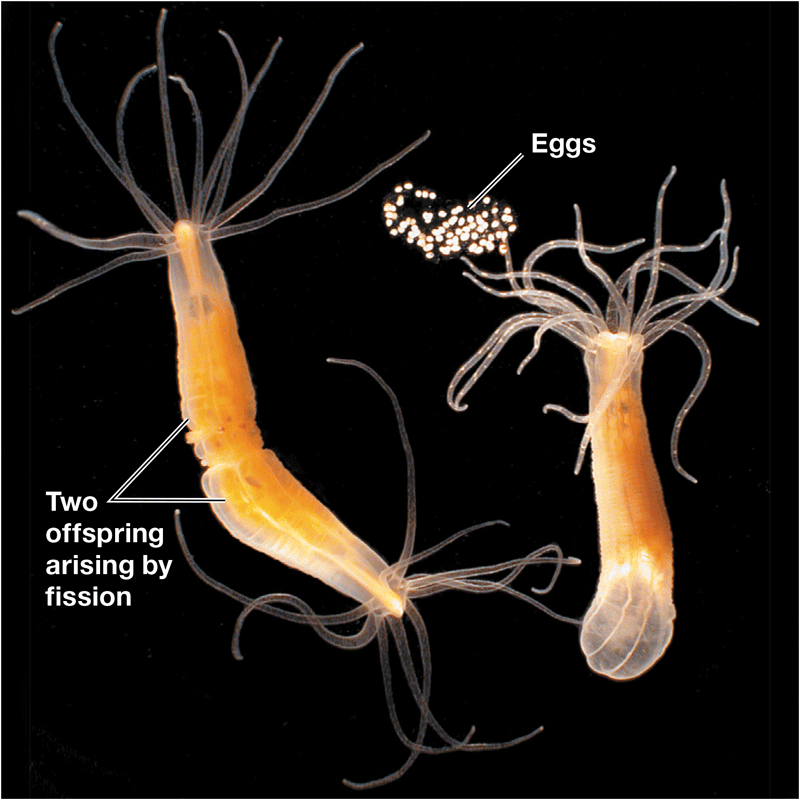
\includegraphics[width=\linewidth]{hermaphroditism.png}
	\caption{The utilization of both asexual and sexual reproduction in the hydra.}
\end{wrapfigure}


In contrast with asexual reproduction, sexual reproduction increases genetic
diversity in the resulting population through random fertilization and
meiosis. The combination of these randomization factors results in the
principal force of natural selection: genetic variability.

While the aspect of variability associated with sexual reproduction might be
attractive for various mobile species, for isolated or immobile organisms,
sexual reproduction is implausible, as it requires a mate with which to
procreate. This inconvenience is addressed by the development of
\textbf{hermaphroditism}, or the existence of both female and male
reproductive systems in a single organism---``perfect'' flowers with both
stamens and carpels, are an example of such a development. The development
of hermaphroditism can be seen as advantageous, as it allows for animals to
reproduce with respect to environmental conditions.

Even with respect to sexual reproduction, there exist two separate development
of reproductive mechanisms: \textbf{reproduction by external fertilization}
wherein gametes are released into and fuse in the environment, and
\textbf{reproduction by internal fertilization} wherein sperm are deposited in
or near the female reproductive tract.

\section{The human female reproductive system}

\begin{wrapfigure}{l}{0.5\textwidth}
	\centering
	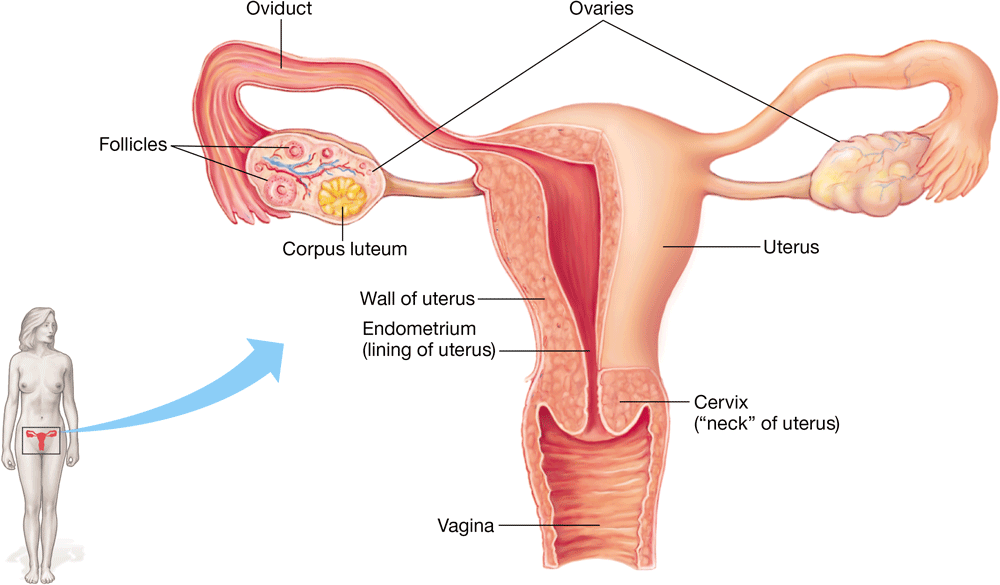
\includegraphics[width=0.9\linewidth]{female_reproductive_system.png}
	\caption{A diagram of the female human reproductive system.}
\end{wrapfigure}

The \textbf{ovaries} are the gamete-producing organs in the female reproductive
system, and can be described as having a ``bumpy'' surface---caused by the
\textbf{follicles} that both produce estrogen and enclose a developing egg cell.

In the process of \textbf{ovulation}, a female will release an immature egg via the
cilia lining the \textbf{oviduct}, or \emph{fallopian tube}---
after starting puberty, of course---as a result of the maturation of a follicle,
every 28 days. In addition, after having matured and formed the \textbf{corpus luteum},
a follicle will begin to release progestrone, alongside additional estrogen, complementing
the maintainence of the uterine lining. This process usually ceases near the age of 50.

With consideration to the above structural definitions, the following statements
regarding the development of a zygote, and the eventual birth of a human fetus
can be made:

\begin{enumerate}
	\item When ovulation occurs, if sperm are present in the upper part of the oviduct,
		fertilization may occur.
	\item After fertilization occurs, the zygote should continuously divide as it traverses
		the oviduct, eventually becoming an embryo.
	\item In the \textbf{uterus}---the site of
		pregnancy\footnote{In rare cases, an \textbf{ectopic pregnancy} may
		commence, where an embryo implants itself in the oviduct, potentially
		rupturing surrounding tissues.}---, an \textbf{embryo} will be
		deposited in the inner lining of the uterus \textbf{endometrium}.
	\item After implantation, the embryo will complete development until the 8th week of
		pregnancy, when the developing human will, henceforth, be referred to as a
		\textbf{fetus}.
	\item After continued development of the fetus, the \textbf{vagina} will serve as the
		canal through which the baby is born. The vagina is separated from the uterus by
		the \textbf{cervix}---the ``neck'' of the uterus.
\end{enumerate}

In addition to each of the aforementioned structures utilized in embryonic and
fetal development, various external structures collectively referred to as the
\textbf{vulva} provide functionality in
copulation\footnote{The \textbf{hymen} could be categorized as one such structure,
but provides little functionality in reproduction, and is ruptured in vigorous
physical activity or intercourse.}:

\begin{itemize}
	\item In sexual intercourse, the \textbf{vagina} serves as a repository for sperm, and
		is guarded by the \textbf{labia minora} and \textbf{labia majora}.
	\item Though it does not provide additional \emph{necessary} functionality in
		reproduction, the \textbf{clitoris}---an erectile organ consisting of a short shaft,
		followed by the \textbf{prepuce}, a small hood of highly sensitive skin---does serve
		a purpose in reproduction in that it evokes a highly presurable sensation when
		stimulated. As do the vagina and th elabia minor, this organ enlarges during sexual
		activity as a result of increased concentration of blood in the area.
\end{itemize}

\section{The human male reproductive system}

As is the case with many other mammals, the natural temperature of the human body presents a
challenge for the proper development of sperm cells within the \textbf{testes}---the male
gonads. That is, in humans, the most desirable temperature for sperm development is
approximately 2\textdegree{C} less than the normal human body temperature of
36.5--37.5\textdegree{C}. In humans, the \textbf{scrotum} solves this dilemma by keeping
sperm-forming cells within the acceptable temperature range.

After a sufficient volume of sperm cells have been produced in the testes, sperm leave
the gonads through the \textbf{epididymis}, where sperm cells will continue to develop
until \textbf{ejaculation}. Once the muscular contractions necessary for ejaculation to
occur take place, the sperm will leave the epididymis via the \textbf{vas deferens}, and
travel upward around the bladder, where the vans deferens joins with the \textbf{seminal
vesicle}. Finally, sperm will be conveyed via the urethera. Thus, it follows that, in
contrast with the female reproductive system, the male reproductive system is directly
related and physically connected to the uninary system. This entire process is
controlled by FSH and LH hormones, and, by extension, the hypothalamus. The former of
the aforementioned hormones, FSH stimulates sperm production, while LH promotes
androgen secretion.

However, the important distinction between sperm and nourishing fluid contained in
semen must be made: \textbf{grandular secretions} are produced by the \textbf{prostate
gland}, and are initially separate from sperm. Alongside \textbf{alkaline mucus}
produced by the \textbf{bulbourethral glands} and sperm, these fluids comprise
\textbf{semen}, the fluid ejaculated from the penis during orgasm.

As does the female reproductive system, the male reproductive system consists of
various external structures:

\begin{itemize}
	\item The \textbf{scrotum}: stores sperm at a suitable temperature
	\item The \textbf{penis}: similarly to the clitoris, this organ is composed
		of erectile tissue forming a shaft, supporting a sensitive glans, and
		is engorged during sexual arrousal\footnote{In individuals with
		\textbf{erectile dysfunction (ED)}, or a tendency to \textbf{impotence},
		engorement of the penis is made improbable. This condition can result from
		drug use, alcohol, or psychological problems.}
\end{itemize}

\begin{figure}[h]
	\centering
	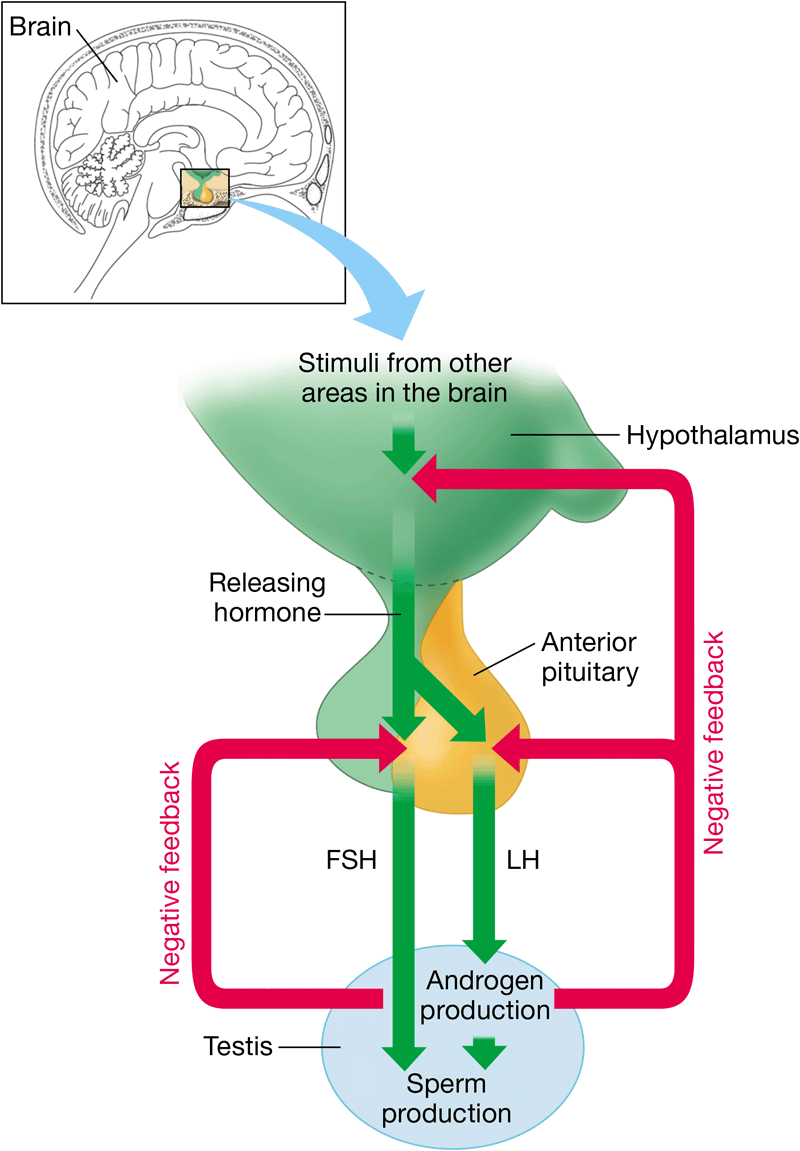
\includegraphics[width=.4\linewidth]{hormonal_control.png}
	\caption{Hormonal control of the testis by the hypothalamus}
\end{figure}

\section{The production of gametes via meiosis}

\begin{wrapfigure}[30]{r}{0.4\textwidth}
	\centering
	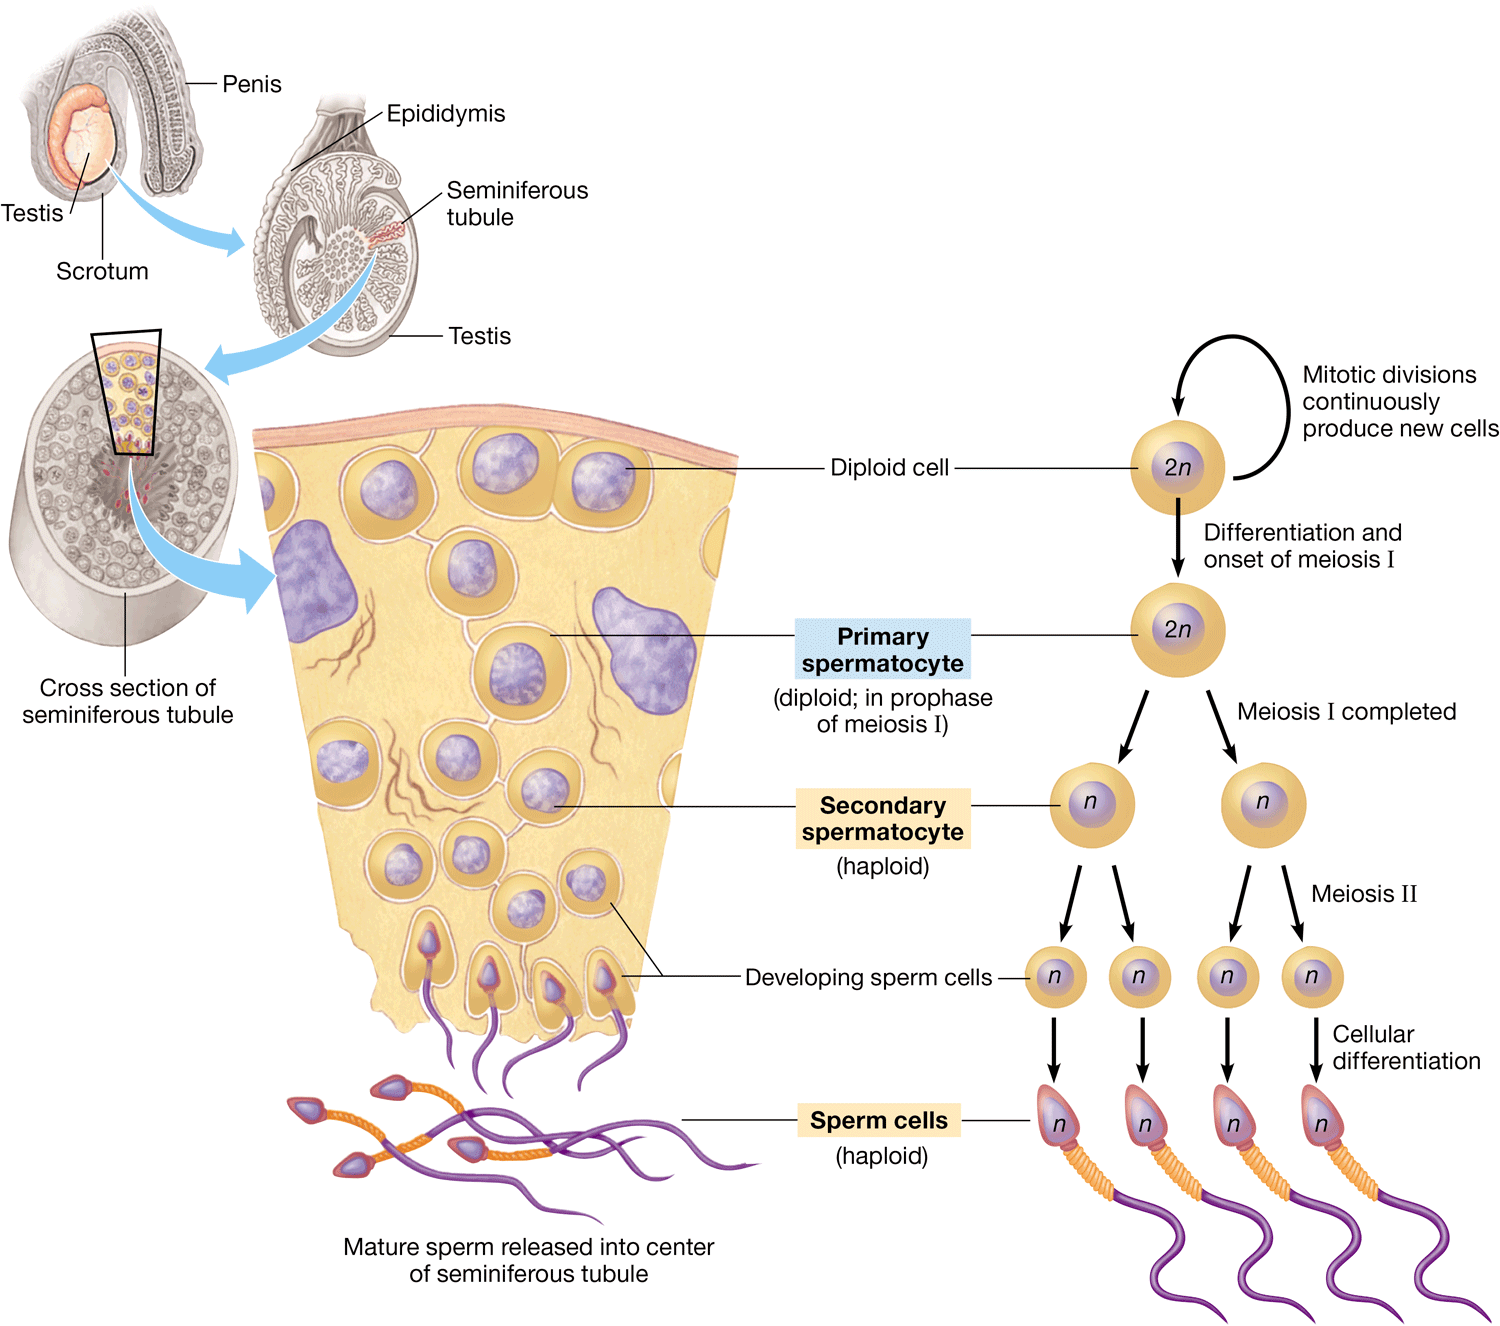
\includegraphics[width=\linewidth]{spermatogenesis.png}
	\caption{The production of gametes in a human female (spermatogenesis).}

	\bigbreak

	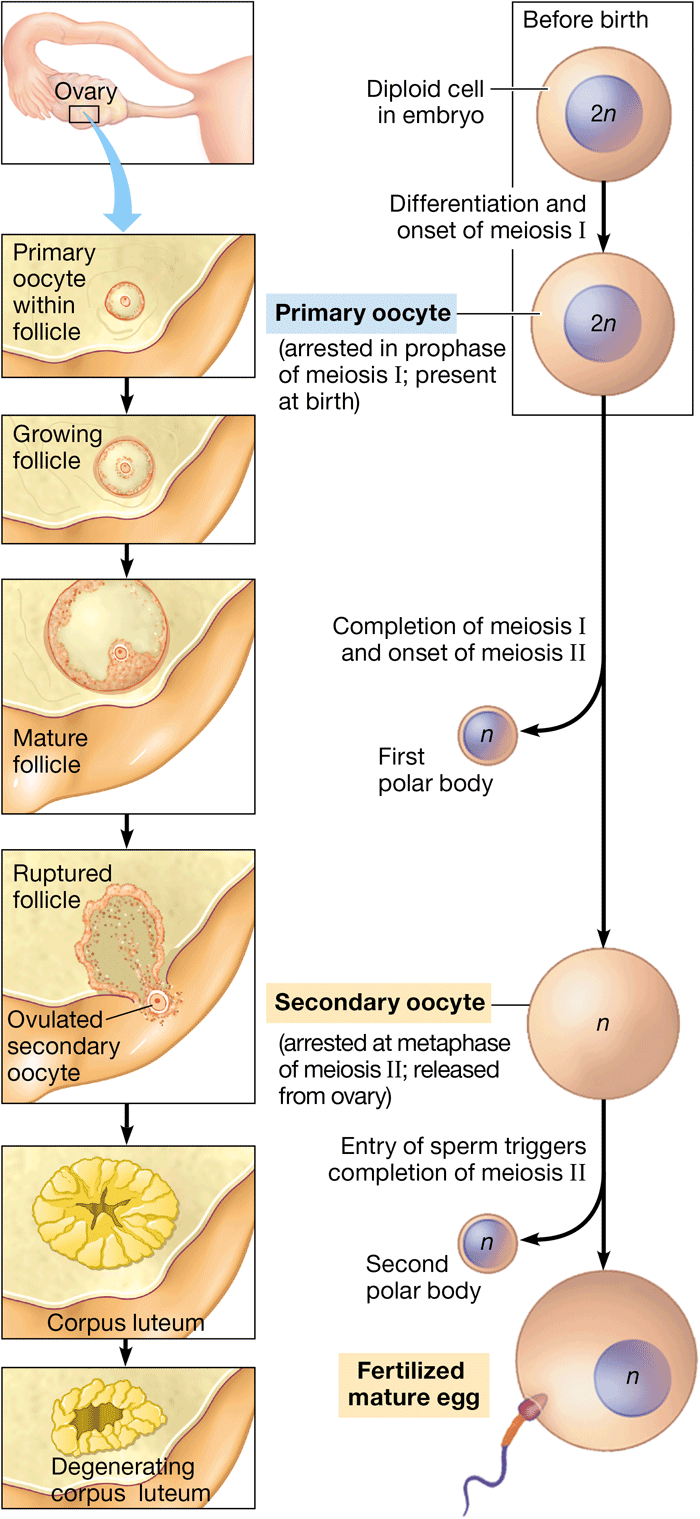
\includegraphics[width=0.4\linewidth]{oogenesis.png}
	\caption{The production of gametes in a human female (oogenesis).}
\end{wrapfigure}

Both egg and sperm cells must be produced through the procedure of meiosis, or
\textbf{gametogenesis}.

\subsection{Spermatogenesis}

\textbf{Spermatogenesis}, or the formation and development of sperm cells,
necessitates the conversion of initially diploid cells ($2n$) in the outer
walls of the coiled seminiferous tubules of the testis to secondary haploid
spermatocytes ($n = 23$). In human males, this process takes approximately
10 weeks to complete, and is usually continuous through the entirety of a
male's adult life.

\subsection{Oogenesis}

\begin{wrapfigure}{R}{0.35\textwidth}
	\centering
	\caption{The production of gamete cells in a human female (oogenesis).}
\end{wrapfigure}

As is the case in spermatogenesis, in oogenesis, the majority of gamete
production and development takes place in the respective gonad---the
ovary. However, in contrast to that which was demonstrated by the male
reproductive system, the female reproductive system does not produce
gametes ``on-demand''---that is, the gametes are produced on a regular
basis, each 28 days, on the basis of the release of a follicle-
stimulating hormone (FSH). This process is, in part, reminiscent of
sperm production, as it is ultimately riggered by the hypothalamus.
However, these two mechanisms do, of course, differ in the fact that:

\begin{enumerate}
	\item Oogenesis occurs in a cyclic fashion, while spermatogenesis
		will be triggered by sexual stimulation
	\item Oogenesis is only carried out between puberty and menopause,
		while spermatogenesis usually lasts the entirety of a male's
		adult life
	\item Naturally, oogenesis produces far less gamete cells than
		spermatogenesis, simply due to the mechanical stipulations
		of human sexual reproduction
\end{enumerate}

The end result of each of these processes is, of course, a haploid
gamete cell.

\section{The female mammalian reproductive cycle is coordinated by hormone secretion}

\subsection{Important distinctions between mammalian reproductive cycle subprocesses.}

The female mammalian reproductive cycle can be divided into two distinct subproceesses:
the \emph{ovarian} cycle and the \emph{menstrual} cycle.

The former of these processes deals exclusively with the production of gamete cells,
while the latter deals with the preparation of the female reproductive system for the
potential implantation of an embryo. Messaging via the exchange of hormones between these
processes allows for the production of gamete cells with respect to a uterine lining
conducive to the growth of an embryo. More specifically, LH and FSH hormones act to
mediate this synchronization effect.

\pagebreak

\subsection{Overview: The female mammalian reproductive cycle}

\begin{wrapfigure}{l}{0.425\textwidth}
	\centering
	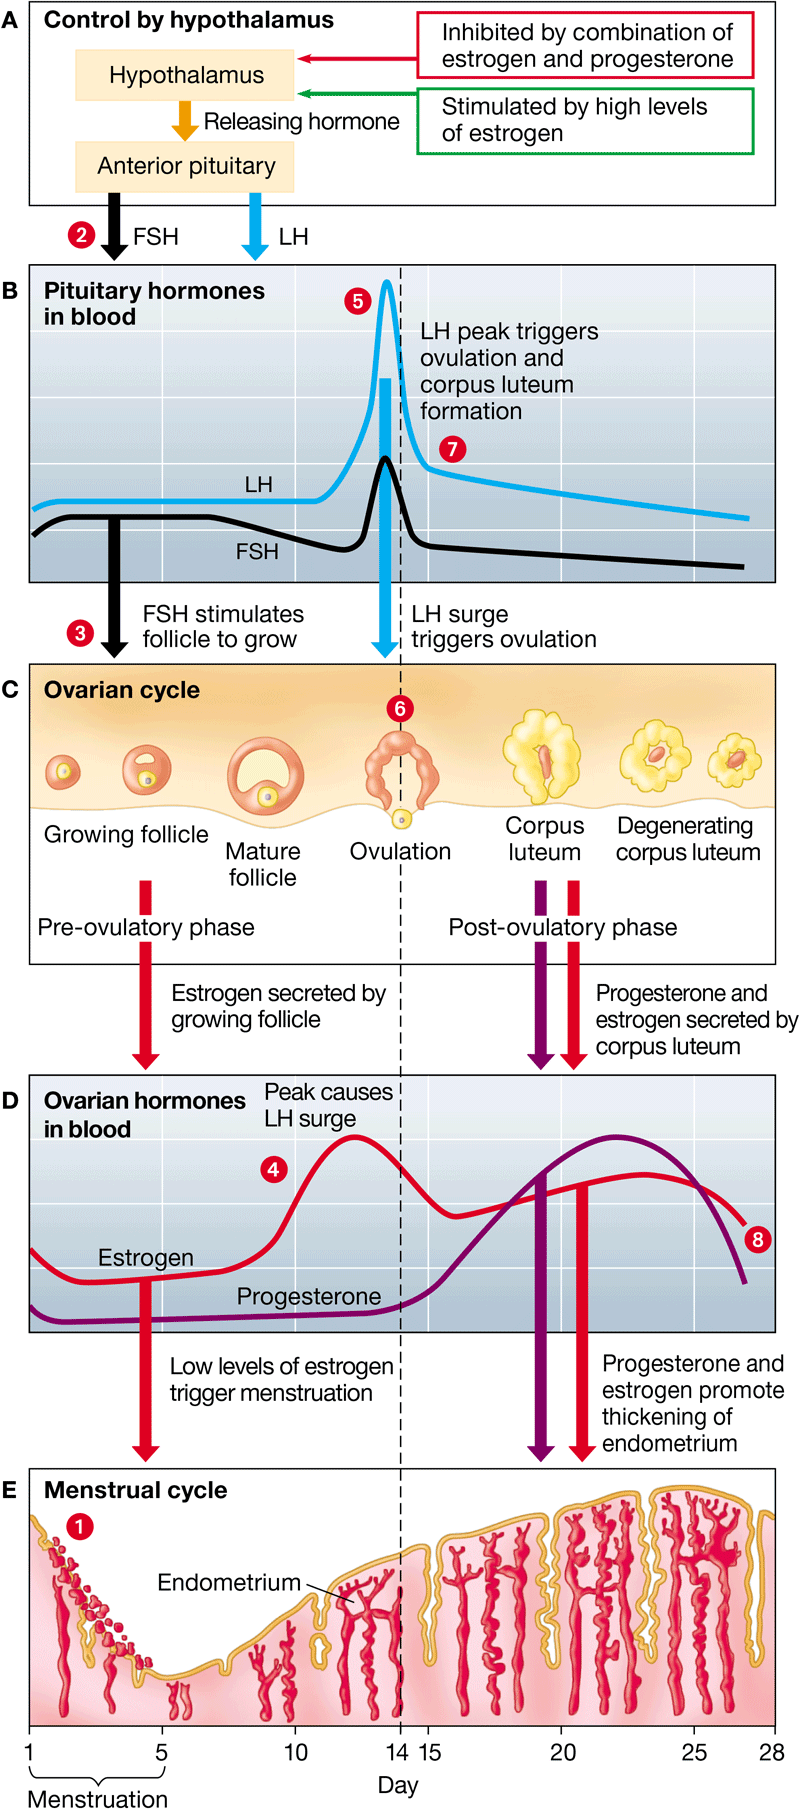
\includegraphics[width=\linewidth]{reproductive_cycle_hormonal_control.png}
	\caption{The reproductive cycle of the human female.}
\end{wrapfigure}

With respect to the discharge of ovules from the ovaries, the ovarian and
menstrual cyclese can be separated into two distinct parts:

\begin{itemize}
	\item The pre-ovulatory phase: the period in which a follicle begins
		growth
	\item The post-ovutory phase: the period in which the follicle has
		become a corpus luteum
\end{itemize}

Typically, when accounting for each of these ``parts'' of the reproductive cycle,
the following sequence of structural events takes place:

\begin{enumerate}
	\item \textbf{Menstruation}: for 3--5 days, the endometrium is in a breakdown
		process, resulting in uterine bleeding. This even occurs at the same time
		as the pre-ovulatory phase of the ovarian cycle.
	\item The endometrium begins to regrow.
	\item After 20--25 days, if the
		embryo has not implanted itself in the uterine lining, the ovarian and menstrual
		cycles restart.
\end{enumerate}

FSH, LH, progesterone and estrogen are the primary hormones responsible for
synchronizing the ovarian and menstrual cycles. The functions of each of the
aforementioned hormones in coordinating the reproductive cycle are as follows:

\begin{itemize}
	\item \textbf{FSH}, or follicle-stimulating hormone: prompts the growth of
		a follicle in the ovaries. In other words, this hormone kicks off the
		ovarian cycle
		\begin{itemize}
			\item Follicles produced as a result of the secretion of FSH
				themselves secrete estrogen, preventing bloodstream
				concentration of FSH and LH low during the pre-ovulatory
				phase
		\end{itemize}
	\item \textbf{Estrogen}: As the period of ovulation approaches and the
		size of the follicle continues to increase, estrogen levels increase
		dramatically. This results in the secretion of FSH and LH en masse.
	\item \textbf{LH}: stimulates the completion of meiosis I, marking the
		production of the secondary oocyte, when the follicle is ruptured.
		\begin{itemize}
			\item Encourages estrogen secretion by the corpus luteum.
		\end{itemize}
	\item \textbf{Estrogen and progesterone}: signals to the hypothalamus that
		FSH and LH level ought to drop, preventing a secondary follicle from
		developing. This effect experiences gradual decay, until the end of
		the post-ovulatory phase, at which point an embryo should have been
		implanted into the uterus. In other words, the decay of this effect
		marks the beginning of the next reproductive cycle.
\end{itemize}

\section{The mechanics of fertilization}

\begin{wrapfigure}{r}{.5\textwidth}
	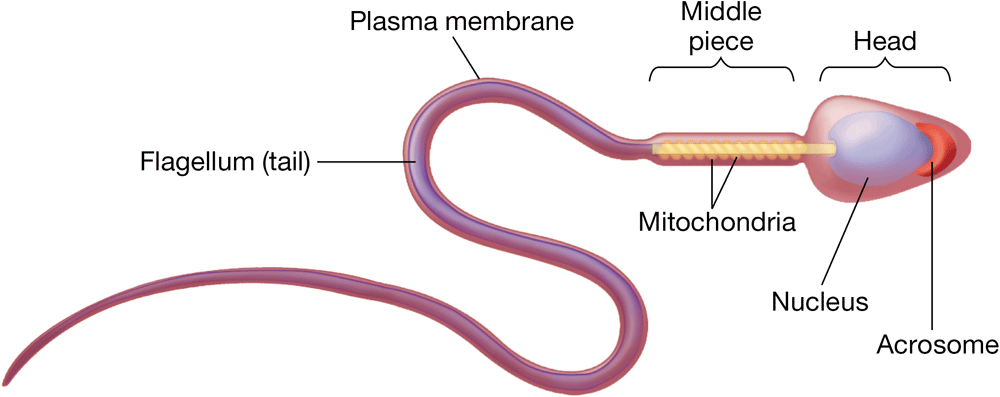
\includegraphics[width=\linewidth]{sperm_cell.png}
	\caption{The structure of a human sperm cell.}
\end{wrapfigure}

Fertilization is, of course, the first step in the development of an embryo---
that is to say, the fusion of two haploid cells from two different individuals
is required in order for the normal pathway of embryo development to ensue.

It is needless to say that the action of fertilization is not inherently
probabilistic: each actor---the sperm cell and the egg cell---
participating in the conjoinment of genetics posess certain properties 
that make fertilizatiion possible. The sperm cell, for example, is
composed of a plasma-membrane enclosed haploid nucleus, an
\textbf{acrosome} containing enzymes that help penetrate the
surface of the egg cell, a flagellum tail, and mitochondria.

With consideration to the biological theme of correlation between structure
and function, it follows that the components found in a typical sperm cell
serve some purpose in fertilization. Thus, one must turn to the natural
process of fertilization itself:

\begin{enumerate}
	\item The sperm cell traverses the uterus, and, eventually, the
		fallopian tubes, utilizing its mitochondria and flagellum tail
	\item A sperm cell binds to an egg cell
	\item The plasma membrane of the cell that will be fertilized becomes
		impenetrable
	\item The vitelline layer of the egg becomes impenetrable
	\item The fusion of the egg and the sperm nuclei is complete
	\item DNA synthesis begins
	\item The zygote divides
\end{enumerate}

\begin{figure}[h]
	\centering
	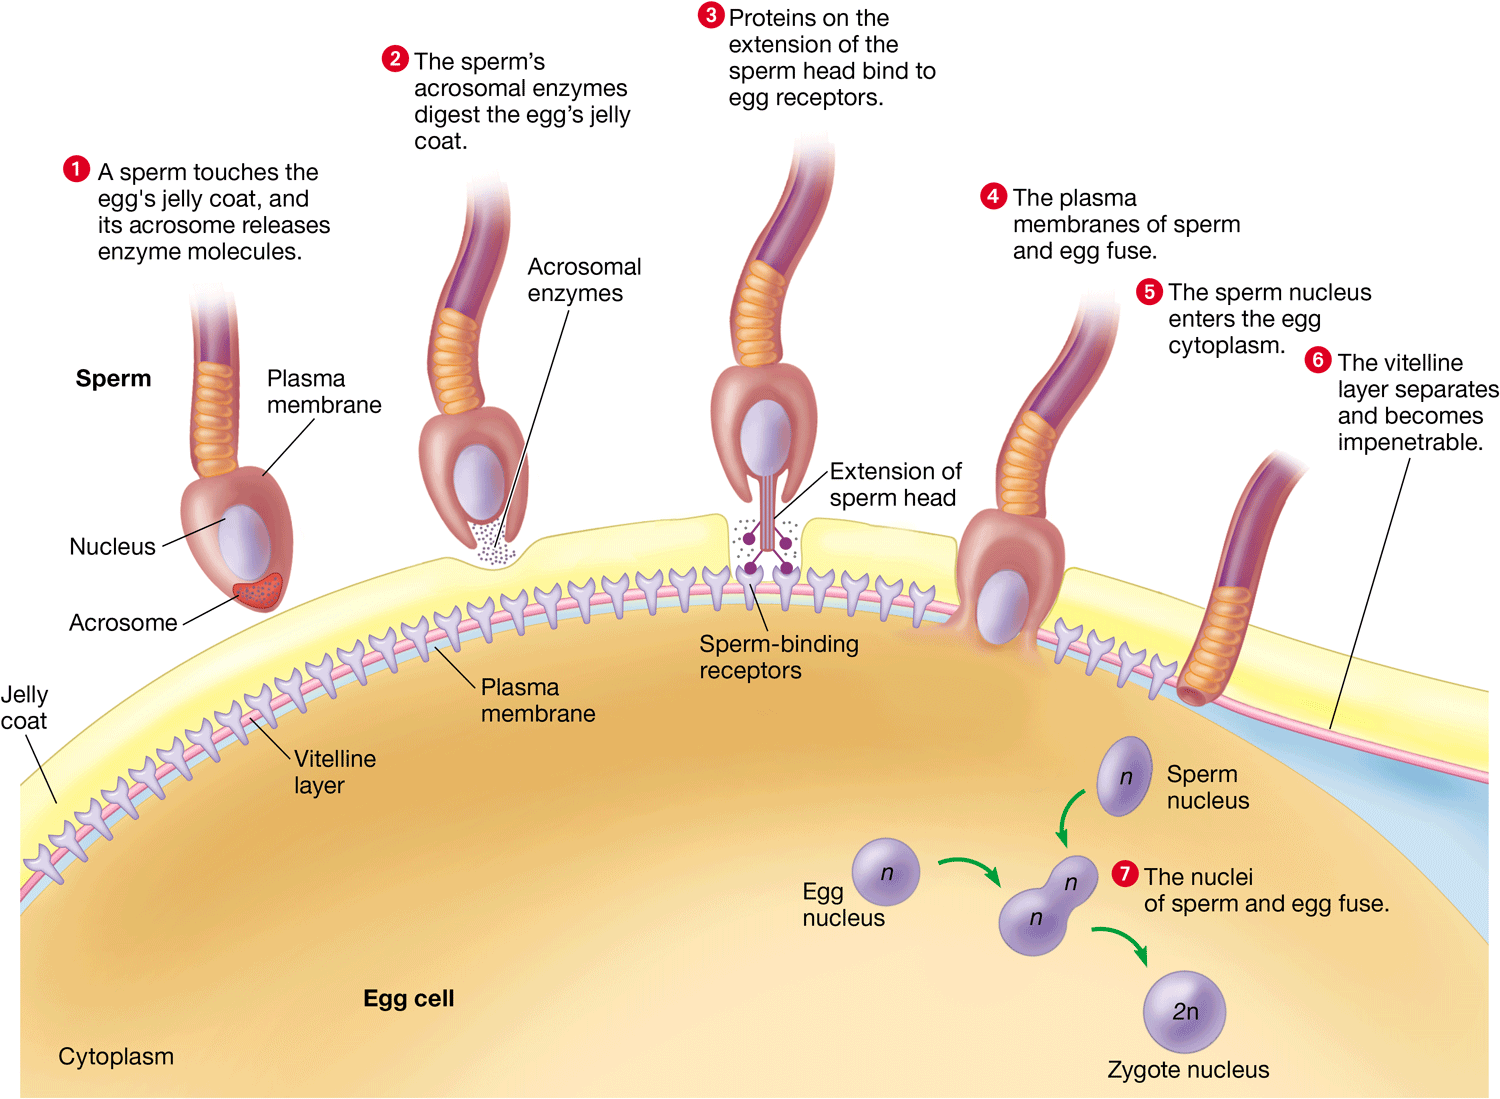
\includegraphics[width=.65\linewidth]{urchin_fertilization.png}
	\caption{The process of fertilization in a sea urchin}
\end{figure}

\section{The mechanics of cleavage}

\textbf{Cleavage} is defined as the first stage in a series of carefully
controllled cell divisions and specialization ultimately leading to the
maturation of an organism. More specifically, cleavage is the stage
during which rapid successive divisions of a zygote lead to the production
of a ``multicellular ball.'' Or, in other words, the completion of this
process results in the transformation of the zygote into an embryo.

It should be noted that, at this point in development, the zygote cell
divides simply for the sake of dividing---that is, division is not performed
with the intention of producing differentiated, or specific \emph{types}
of cells. Furthermore, the zygote does not produce many new proteins at this
point, and simply seeks to sustain division by feeding off nutrients stored in
the containing egg. Yet, with consideration to the non-expansionist manner of
development at this stage in maturation, it remains true that this action of
``division'' is less akin to traditional mitosis, and bears more resemblance
to the simple action of \emph{partition}---new cells are not significantly
larger than---or even comparable in size, for that matter, with consideration
to---the source cell.

Typically cleavage takes approximately 4 hours to complete in a frog, and 4
days to complete in a human.

One notable development that arises about the completion of cleavage is the
formation of the \textbf{blastocoel}---a fluid-filled cavitiy located in the
center of the embryo. After the completion of cleavage, this cavity transforms
into a \textbf{blastula}, a hollow ball of undifferentiated cells that pose
quite promising therapeutic use cases.

\section{The mechanics of gastrulation}

\begin{wrapfigure}{R}{.4\textwidth}
	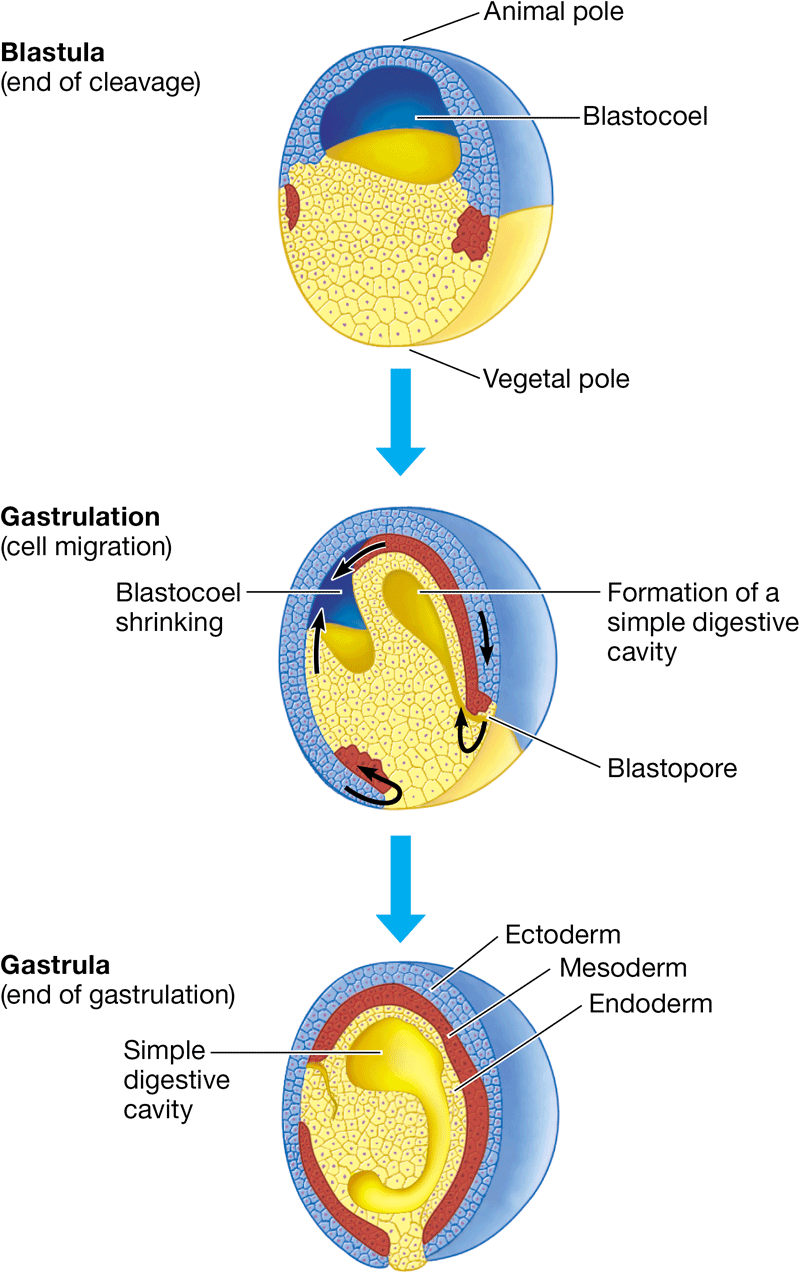
\includegraphics[width=\linewidth]{frog_gastrulation.png}
	\caption{Gastrulation in a frog.}
\end{wrapfigure}

\textbf{Gastrulation}, the second phase of embryonic development, is perhaps
best likened to a blueprinting phase of maturation---that is, cells are
arranged in a manner that is conducive to the efficient formation of further
organs and tissues. This ``wireframing / blueprinting'' action results in the
formation of a \textbf{gastrula}, or a three-layer stage. The three stages
comprising the gastrula can be defined as such:

\begin{itemize}
	\item \textbf{Ectoderm}: the outer layer of the gastrula---likened to the
		epidermis of the adult skin, the epithelial lining of the mouth and
		rectum, the sense receptors in the epidermis, the cornea and lens of
		the eye, and the nervous system
	\item \textbf{Endoderm}: represents the digestive tract of an embryo---likened
		to the epithelial lining of both an adult digestive tract and respiratory
		system, the liver, the pancreas, the thyroid, the parathyroids, the thymus,
		the lining of the urethera, the urinary bladder, and the reproductive system
	\item \textbf{Mesoderm}: lies between the two aforementioned ``sections'' of the
		embryonic developmental stage---akin to the skeletal, muscular, circulatory,
		excretory, and reproductive systems
\end{itemize}

\section{The mechanics of organ development}

Following the ``blueprinting'' phase of embryonic development, several new organs
will arise in the embryo:

\begin{itemize}
	\item The \textbf{nortochord}
	\item The \textbf{neural folds}
	\item The \textbf{neural plate}
\end{itemize}

However, the distinction should be made that the aforementioned organs are not in
and of themselves organs in the traditional sense of the word. The nortochord,
for example, develops in the mesoderm, but does not serve any function other than
of a glorified ``play-doh'' kit: it can be molded and fitted into any organ that
arises in the same ``section'' of the embryonic stage: the nerve cord, for example,
begins to form as a derivative structure of the nortochord at this point in
maturation. Usually, a large part of this structure will dissolve before birth,
though parts of the adult spine might bear composure from the nortochord.

As does the nortochord, both the neural folds and the neural plate eventually
fade into the structural composition of the resultant embryo: the neural plate
is ``rolled'' transformed by various rolling and sinking actions into what
becomes the \textbf{neural tube}---the adult brain and spinal cord.

At this point, in various animals---frogs, for example---, the \textbf{coelom}
will begin to form. In addition to the aforementioned structures, the body
cavity or coelom represent some of the fundamental features of all chordates.

\bigbreak

\begin{figure}[h]
	\centering
	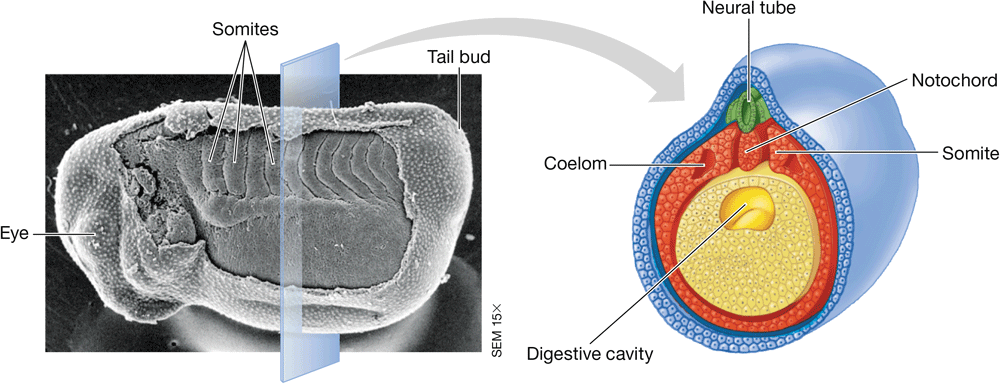
\includegraphics[width=.8\linewidth]{embryo_cross_section_neural_tube.png}
	\caption{An embryo with completed neural tube, somites, and coelom shown in a side view (left) and in cross section (right)}
\end{figure}

\section{The mechanics of animal development}

So far, several stages in the development of an embryon have been discussed.
Yet, the mechanism by which such coordination occcurs remains unclear. In
practice, these developmental stages come about through the coordination of
various, interconnected processes through \textbf{induction}---the influence
of one group of cells on an adjacent group of cells. Of course, induction may
be carried out through various kinds of communication. Cell-surface interaction
is one such mode of communication.

In the development of organ cells, for example, the aforementioned coordination
techniques are utilized: in order to be differentiated into specific types of
tissues, a set of genes must be ``switched on'' through induction.

While induction does play a heavy role in various embryonic developmental processes,
\textbf{cell migration} also plays a non-discountable role in gastrulation, for
example: cells within the embryo ``crawl'' by extending and contracting in accordance
with the aforementioned induction technique.

Finally, \textbf{apoptosis}, or cell suicide, allow ``spaces'' to be hollowed
out in an organism, should the need arise.

\begin{figure}[h]
	\centering
	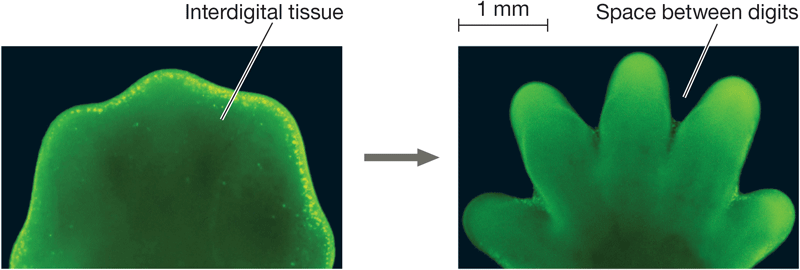
\includegraphics[width=.8\linewidth]{mouse_paw_apoptosis.png}
	\caption{Apoptosis in a developing mouse paw}
\end{figure}

\section{The mechanics of gestation}

Approximately 24 hours after conception, a \textbf{blastocyst}, or sphere of
undifferentiated cells, forms. This ``ball'' of cells is coated in a layer of
outer cells that comprise the \textbf{trophoblast}, which secretes enzymes
conducive to the implantation of the embryo in the uterine lining.

The process of implantation itself relies on the extension of trophoblast cells
onto the endometrium. Having said so, these ``extension'' cells eventually form
the \textbf{placenta}---a nourishing organ for the embryo. Alongside the placenta,
various \textbf{extraembryonic membranes}---the amnion, the yolk sac, and the chorion
---will form, each helping support the embryo.

\bigbreak

\begin{figure}[h]
	\centering
	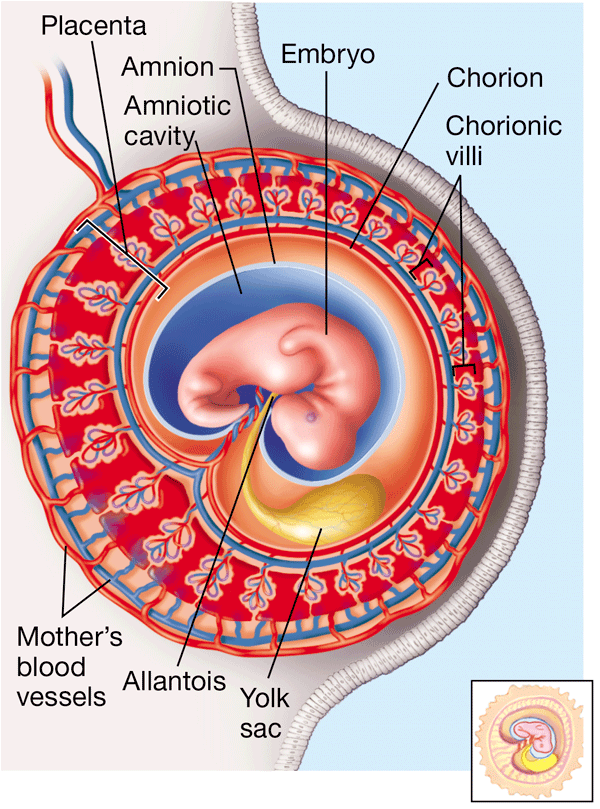
\includegraphics[width=.475\linewidth]{placenta.png}
	\caption{The embryo 31 days after conception.}
\end{figure}

\section{The mechanics of childbirth}

In order for \textbf{labor}, or the seris of events that expel an infant from
the uterus to occur, various hormones must be present in the mother's body,
in order to illicit their respective responses from the body:

\begin{itemize}
	\item Estrogen: triggers the formation of oxytocin receptors inside the uterus,
		resulting in the rhythmic contractions associated with labor 
	\item Prostaglandin: stimulate the contraction of the uterine muscle cells
\end{itemize}

With consideration to each of the aforementioned factors, the process of labor may
begin:

\begin{enumerate}
	\item \textbf{Dilation}: lasts 6-12 hours, from the initiation of the labor
		process until a maximum dilation of 10 cm
	\item \textbf{Expulsion}: infant is forced down and out of the uterus and vagina
	\item \textbf{``Afterbirth''}: umbilical cord is severed
\end{enumerate}

\begin{figure}[h]
	\centering
	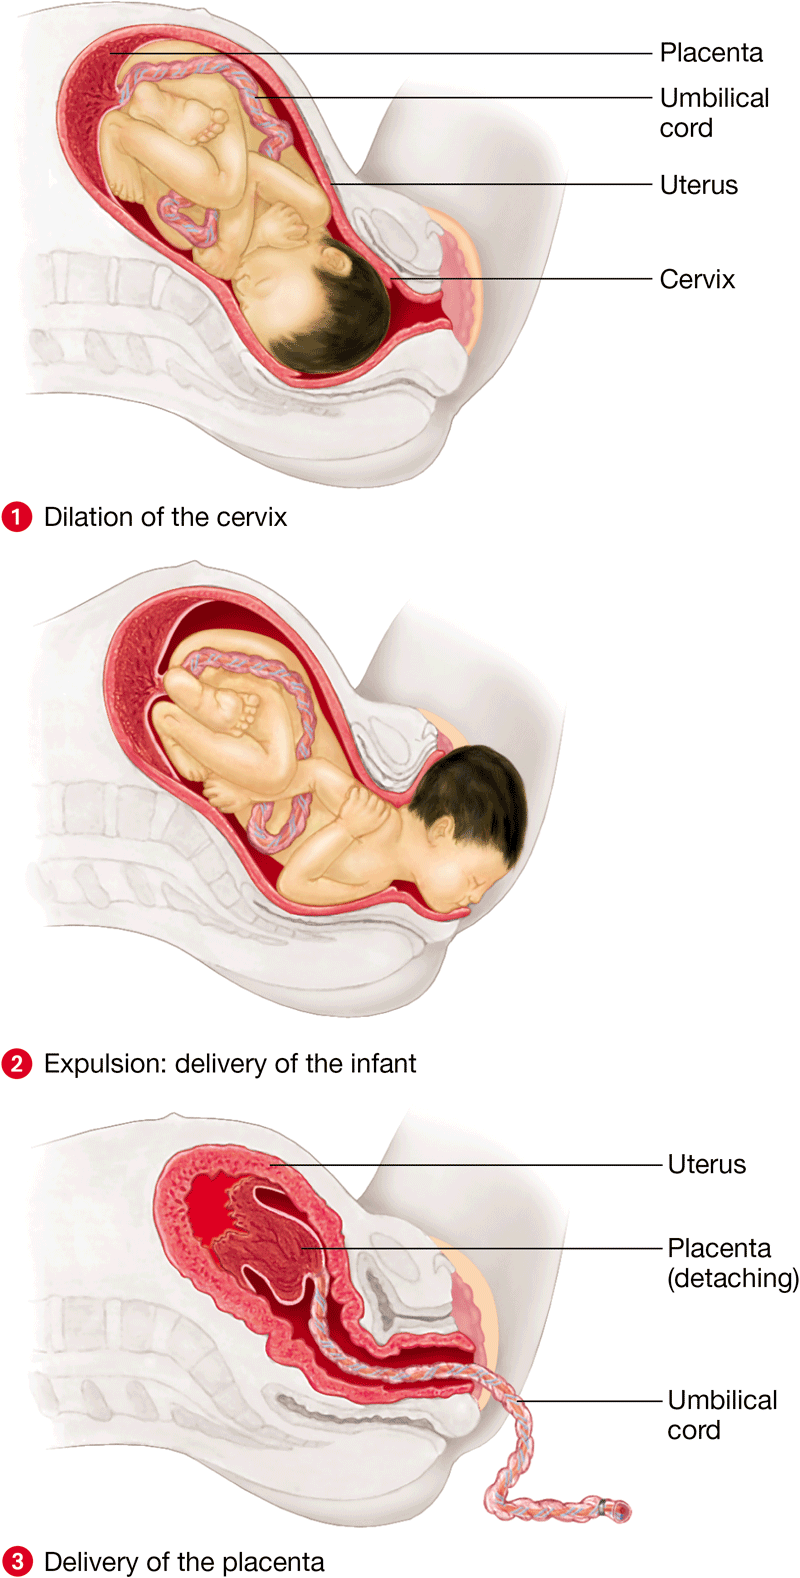
\includegraphics[width=.45\linewidth]{infant_delivery.png}
	\caption{The three stages of labor}
\end{figure}

\end{document}
